% Set Title, Author, and email
\title{DCO1013 - canal dispersivo}
\author{Levy Gabriel da S. G. \\ Engenharia elétrica - UFRN}

\maketitle
\thispagestyle{fancy}

Segundo as considerações impostas pelo exercício, a saída y(t) do canal será:

\begin{center}
    $y(t) = g(t) \ast h(t)$
\end{center}

No domínio tem-se:

\begin{center}
    $Y(f) = G(f) \ast H(f)$
\end{center}

Onde $G(f)\rightleftharpoons g(t)$ representa o sinal sujeito ao canal, $H(f)$ o canal e $Y(f)$ a saída do canal. Assim, desenvolvendo a equação baseado na definição do canal:

\begin{center}
    $Y(f) = G(f)e^{-j2\pi f t_d} + k \, cos(2\pi fT) G(f)e^{-j2\pi f t_d}$
\end{center}

De acordo com a fórmula de Euler, o cosseno pode ser expresso como uma soma de exponenciais no domínio em questão (no caso da frequência):

\begin{center}
    $cos(2\pi f T) = \frac{1}{2} (e^{j2\pi f T}   +    e^{-j2\pi f T})$
\end{center}

Incorporando essa expressão à equação da saída $Y(f)$:

\begin{center}
    $Y(f) = G(f)e^{-j2\pi f t_d} + \frac{k}{2} \, G(f)   [e^{-j2\pi f (t_d-T)}   +    e^{-j2\pi f (t_d+T)}]$
\end{center}

Considerando a propriedade de deslocamento no tempo da transformada de Fourier para um deslocamento genérico $x$: $G(f)e^{-j2\pi f x} \rightleftharpoons g(t-x)$. Com isso pode-se determinar a expressão do tempo na saída por meio dessa propriedade considerando valores de atraso para $x$ como $t_d$, $t_d-T$ e $t-d+T$, assim a expressão para a saída será:

\begin{center}
    $y(t) = g(t-t_d) + \frac{k}{2} [g(t-t_d+T) + g(t-t_d-T)]$
\end{center}

Outra forma de enxergar essa expressão é fazer $t=t+t_d$:

\begin{center}
    $y(t+t_d) = g(t) + \frac{k}{2} [g(t+T) + g(t-T)]$
\end{center}

Isso permite observar que a saída é a ponderação acima baseada na função $g(t)$ atrasada de $t_d$.

Para ilustrar a forma de onda, não será considerada a forma de onda genérica de $g(t)$ como aquela apresentada no problema, mas sim uma forma modificada para facilitar a representação gráfica, como a da figura \ref{graph:1}.


\begin{figure}[H]
\centering

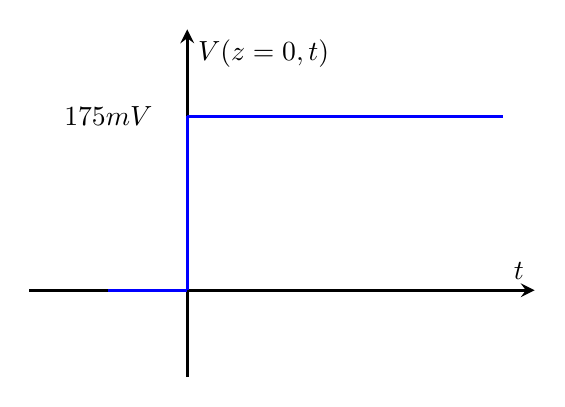
\begin{tikzpicture} 
\begin{axis}[very thick,
                     samples = 100,
                     ytick={-2,2},
                     xlabel = {$t$},
                     ylabel = {$V(z=0, t)$},
                     xmin = -1,
                     xmax = 2.2,
                     ymin = -0.5,
                     ymax = 1.5,
                     width=8cm,
                     height=6cm,
                     axis x line = middle,
                     axis y line = middle,
                     ticks = none]
                     
            \addplot[blue] coordinates {(-0.5,0) (0,0)};
            \addplot[blue] coordinates {(0,0) (0,1)};
            \addplot[blue] coordinates {(0,1) (2,1)};
            \node at (axis cs:-0.5,1){$175 mV$};
            
        \end{axis}
\end{tikzpicture}

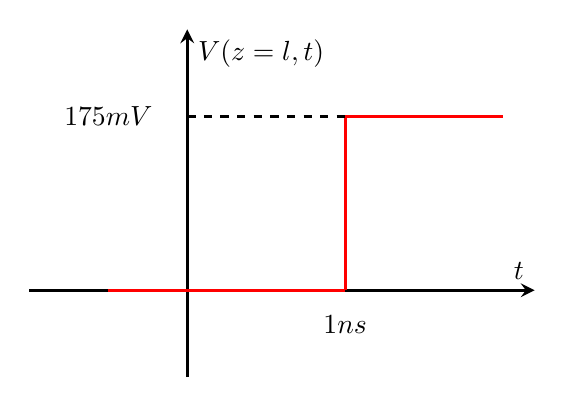
\begin{tikzpicture} 
\begin{axis}[very thick,
                     samples = 100,
                     ytick={-2,2},
                     xlabel = {$t$},
                     ylabel = {$V(z=l, t)$},
                     xmin = -1,
                     xmax = 2.2,
                     ymin = -0.5,
                     ymax = 1.5,
                     width=8cm,
                     height=6cm,
                     axis x line = middle,
                     axis y line = middle,
                     ticks = none]
                     
            \addplot[red] coordinates {(-0.5,0) (1,0)};
            \addplot[red] coordinates {(1,0) (1,1)};
            \addplot[red] coordinates {(1,1) (2,1)};
            \addplot[dashed] coordinates {(0,1) (1,1)};
            \node at (axis cs:-0.5,1){$175 mV$};
            \node at (axis cs:1,-0.2){$1ns$};
            
        \end{axis}
\end{tikzpicture}

\caption{First graph shows the voltage at the start of the line and the second shows the voltage at the end of the line. Source: own.}
\label{graph:1} 
\end{figure}

Assim, a forma de onda da saída será a seguinte composição:


\begin{figure}[H]
\centering
\tikz \node [scale=0.8, inner sep=0] {
\begin{tikzpicture} 
    \draw[black, very thick] (-2,3) -- (0,3);
    \draw[black, very thick] (0,3) -- (0,0);
    \draw[black, very thick] (0,0) -- (2,0);
    \node[blue] at (-2.4,3) {$R_{in}$};  
    \node[red] at (2.4,0) {$R_{L}$};  
    \node[black] at (1,1.5) {$1+Q_s^2$};  
    \draw[>=latex, <->] (0.2,0) -- (0.2,3);
    \node[black] at (0,-0.5) {(a)};
\end{tikzpicture}
};
\hspace{1cm}
\tikz \node [scale=0.8, inner sep=0] {
\begin{tikzpicture} [american]
    \draw[>=triangle 90, ->] (-0.5,0) -- (0.5,0);
    \draw[>=triangle 90, ->] (6.5,0) -- (5.5,0);
    \node[black] at (-0.9,0) {$R_{in}$}; 
    \node[black] at (6.9,0) {$R_L$}; 
    \node[black] at (3,-4) {(b)};
    \draw (1,0) to[L, l=$L$, *-*] (5,0)
    (2,0) to[C, l=$C$, *-] (2,-3) node[ground]{}
    ;
\end{tikzpicture}
};

\caption{(a) Desired effect of impedance gain(b) L matching network for a serial to parallel transformation of load impedance. Source: own.}
\label{graph:2} 
\end{figure}



